%%%%%%%%%%%%%%%%%%%%%%%%%%%%%%%%%%%%%%%%%
% University Assignment Title Page 
% LaTeX Template
% Version 1.0 (27/12/12)
%
% This template has been downloaded from:
% http://www.LaTeXTemplates.com
%
% Original author:
% WikiBooks (http://en.wikibooks.org/wiki/LaTeX/Title_Creation)
%
% License:
% CC BY-NC-SA 3.0 (http://creativecommons.org/licenses/by-nc-sa/3.0/)
% 
% Instructions for using this template:
% This title page is capable of being compiled as is. This is not useful for 
% including it in another document. To do this, you have two options: 
%
% 1) Copy/paste everything between \begin{document} and \end{document} 
% starting at \begin{titlepage} and paste this into another LaTeX file where you 
% want your title page.
% OR
% 2) Remove everything outside the \begin{titlepage} and \end{titlepage} and 
% move this file to the same directory as the LaTeX file you wish to add it to. 
% Then add \input{./title_page_1.tex} to your LaTeX file where you want your
% title page.
%
%%%%%%%%%%%%%%%%%%%%%%%%%%%%%%%%%%%%%%%%%
%\title{Title page with logo}
%----------------------------------------------------------------------------------------
%	PACKAGES AND OTHER DOCUMENT CONFIGURATIONS
%----------------------------------------------------------------------------------------

\documentclass[12pt]{article}
\usepackage[english]{babel}
\usepackage[utf8x]{inputenc}
\usepackage{amsmath}
\usepackage{graphicx}
\usepackage[colorinlistoftodos]{todonotes}
\usepackage{subcaption}

\begin{document}

\begin{titlepage}

\newcommand{\HRule}{\rule{\linewidth}{0.5mm}} % Defines a new command for the horizontal lines, change thickness here

\center % Center everything on the page
 
%----------------------------------------------------------------------------------------
%	HEADING SECTIONS
%----------------------------------------------------------------------------------------

% Name of your university/college
\textsc{\LARGE Instituto Superior T\'{e}cnico}\\[1.5cm]
% Major heading such as course name
\textsc{\Large ISR}\\[0.5cm]
% First Minor heading such as course title
\textsc{\large Report}\\[0.25cm]
% Second Minor heading such as course title
\textsc{\small State Of The Art Milestone}\\[0.25cm]

%----------------------------------------------------------------------------------------
%	TITLE SECTION
%----------------------------------------------------------------------------------------

\HRule \\[0.5cm]
{ \large \bfseries State Of The Art Essay: User Interface Related Work}\\[0.25cm] % Title of your document
\HRule \\[0.5cm]
 
%----------------------------------------------------------------------------------------
%	AUTHOR SECTION
%----------------------------------------------------------------------------------------

\begin{minipage}{0.4\textwidth}
\begin{flushleft} \large
\emph{Author:}\\
Francisco Maria \textsc{Calisto} % Your name
\end{flushleft}
\end{minipage}
~
\begin{minipage}{0.4\textwidth}
\begin{flushright} \large
\emph{Coordinator:} \\
Jacinto \textsc{Peixoto} % Coordinator's Name
\end{flushright}
~
\begin{flushright} \large
\emph{Co-Coordinator:} \\
Daniel \textsc{Gon\c{c}alves} % Co-Coordinator's Name
\end{flushright}
\end{minipage}\\[2cm]

% If you don't want a supervisor, uncomment the two lines below and remove the section above
%\Large \emph{Author:}\\
%John \textsc{Smith}\\[3cm] % Your name

%----------------------------------------------------------------------------------------
%	DATE SECTION
%----------------------------------------------------------------------------------------

{\large 19/04/2016}\\[1cm] % Date, change the \today to a set date if you want to be precise

%----------------------------------------------------------------------------------------
%	LOGO SECTION
%----------------------------------------------------------------------------------------

% 
\includegraphics{ist-logo.png}\\[0.5cm] % Include a department/university logo - this will require the graphicx package

% 
\includegraphics{isr-logo.png}\\[0.5cm] % Include a department/university logo - this will require the graphicx package

\begin{figure}
\centering
\begin{subfigure}{.5\textwidth}
  \centering
  
\includegraphics[width=.5\linewidth]{isr-logo.png}
\end{subfigure}%
\begin{subfigure}{.5\textwidth}
  \centering
  
\includegraphics[width=.5\linewidth]{inesc-id-logo.png}
\end{subfigure}
\begin{subfigure}{.5\textwidth}
  \centering
  
\includegraphics[width=.25\linewidth]{ist-logo.png}
\end{subfigure}
\end{figure}
 
%----------------------------------------------------------------------------------------

\vfill % Fill the rest of the page with whitespace

\end{titlepage}

\section{Introduction}

Doctors are accountable for decisions they make on behalf of their patients. Likewise, Computer Interface Developers and Engineers must assume accountability for limitations, assumptions and other unplanned deficiencies that impact on the integrity, validity, quantity and timeliness of data made accessible through their interfaces.

Art and science of clinical care are based on an unusual combination of non-judgement trust and exasperating mistrust. Doctors and Clinicians require that theirs patients keep no secrets or else an opportunity to reach the right diagnosis or select the proper therapy may be lost. At the same time, doctors and clinicians are taught to question everything they hear from both colleagues and patients. It is deeply ingrained in medical training to make no important decisions based on information supplied solely by others. The highly trained mistrust explains why many times patients complained that a dozen different people asked the same question. A deeply ingrained aversion incorporate the concept of visual accountability extends well beyond medical user interfaces.

The growing interest in multimodal interface development is inspired in large part by goals of supporting more flexible, transparent, efficient and powerfully expressive means of human-computer interaction than in the past. Multimodal interfaces are expected to support a wider range of diverse applications, be usable by a broader spectrum of the average population, and function more reliably under realistic and challenging usage conditions.

To realise successful multimodal systems of the future, may key research challenges remain to be addressed. Among these challenges are the development of effective natural language processing, dialogue processing, and error-handling techniques. In Addition, new multimodal systems will be needed for collaborative multiperson use. Before this new class os systems can proliferate, toolkits also will be needed to promote software development for both simulated and functioning systems.

Multimodal interfaces also are expected to be easier to learn and use, and they are preferred by users for many applications. They have the potential to expand computing to more challenging applications, be used by a broader spectrum of everyday people, and accommodate more adverse usage conditions than in the past. This class of systems represents a relatively new direction for computing that draws from myriad input and output technologies currently becoming available.

\section{Overview}



\section{}



%% Commands to include a figure:
%\begin{figure}[!hbt]
%\centering
%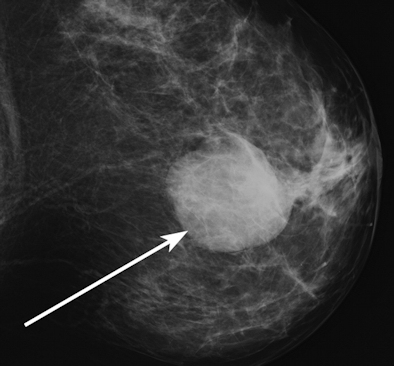
\includegraphics[width=0.75\textwidth]{masses.png}
%\caption{\label{fig:frog}Mammographic image of a high-density mass
%}
%\end{figure}
%
%% Commands to include a figure:
%\begin{figure}[!hbt]
%\centering
%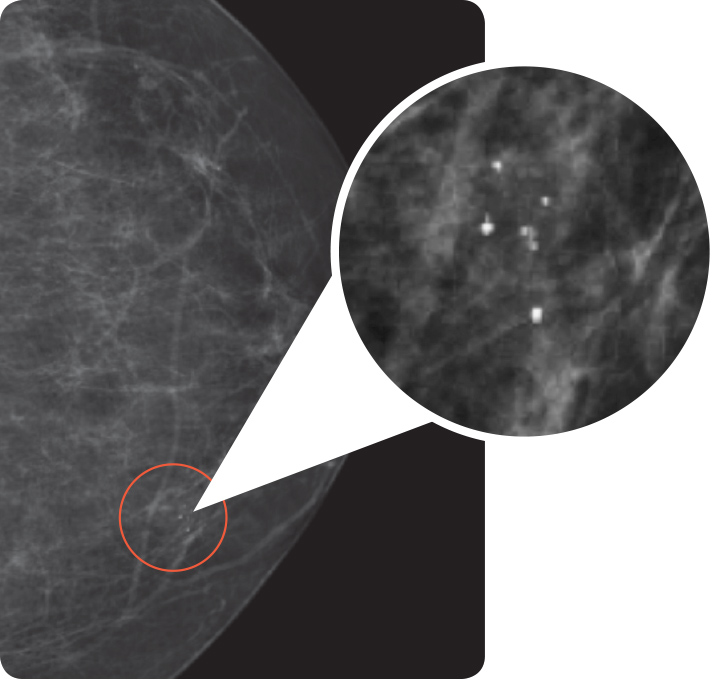
\includegraphics[width=0.75\textwidth]{calcifications.png}
%\caption{\label{fig:frog}Mammogram – shows calcifications, an early sign of breast cancer
%}
%\end{figure}
%
%\clearpage

\section{Related Work}



\subsection{}



\subsection{}

Another direction of work is known as Fine Needle Aspirate (FNA) [23]. Basically, their class of approaches, by using computer based image analysing, we research a Breast Cytology Diagnosis via Digital Image Analysis [1] paper work that brings us an improvement on the diagnostic accuracy of breast FNA goal where an interactive computer system has been developed for evaluating cytologic features derived directly from a digital scan of breast FNA slides. The system uses computer vision technology techniques to analyse cell nuclei and classifies them using an inductive method based on linear programming.

\clearpage



\subsection{}



\subsection{}



\clearpage

\section{}



%% Commands to include a figure:
%\begin{figure}[!hbt]
%\centering
%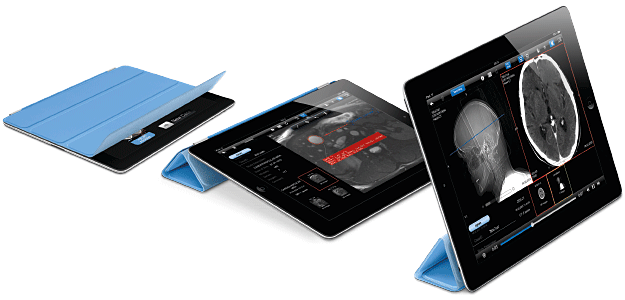
\includegraphics[width=0.75\textwidth]{mobile.png}
%\caption{\label{fig:frog}aycan mobile
%}
%\end{figure}



\clearpage



\section{Conclusions}



\clearpage

\begin{thebibliography}{}


\clearpage



\clearpage


\bibitem{} Arbab Masood Ahmad, Gul Muhammad Khan, Sahibzada Ali Mahmud, and Julian Francis Miller. 2012. Breast cancer detection using cartesian genetic programming evolved artificial neural networks.  In \emph{Proceedings of the 14th annual conference on Genetic and evolutionary computation} (GECCO '12), Terence Soule (Ed.). ACM, New York, NY, USA,  1031-1038. DOI=http://dx.doi.org/10.1145/2330163.2330307
\end{thebibliography}

\end{document}
